\section{Adaptive Mesh refinement}


Em muitos escoamentos de interesse, as estruturas que exigem alto refino de malha, como camada limite, interface entre fluidos e pequenas recirculações, se concentram apenas em locais específicos do domínio e são móveis, sofrendo grandes deformações. Para esses casos, uma malha uniforme com resolução suficiente para capturar tais fenômenos é, principalmente quando o número de dimensões do escoamento aumenta, proibitiva. Diante disto, vários modelos de remalhagem dinâmica foram criados ao longo da literatura, sendo um deles o chamado refinamento de malha adaptativo (adaptive Mesh refinement AMR), um algoritmo introduzido por \cite{Berger1984} que ajusta o refino de malha localmente, com base em valores de truncamento ou gradientes abruptos, e que organiza esses refinos em uma hierarquia formada por blocos de malha aninhados em cada nível de refinamento.

A metologia, consolidada em \citet{Berger1989}, consiste em um sistema de patches de malha e pode ser ilustrado da seguinte forma: Considere por exemplo uma malha uniforme de espaçamento de malha $h$ que cobre todo o domínio, essa malha é considerada um path de malha $G_1$ e pertence ao nível de malha $l_1$. Considere também que existem duas estruturas que exigem níveis de refino maiores que $h$ é necessário a criação de um novo nível de malha, com refino $h_2$ e com patches delimitados por $G_{2,k}$ onde k delimita o número do patch. No algoritmo de malha adaptativa de Berger esse processo se repete iterativamente, para cada nível, de forma que cada nível $l$ precisa estar contido em um nível mais abrangente $l-1$. A Figura \ref{fig:ilustração_AMR}.


\begin{figure}
    \centering
    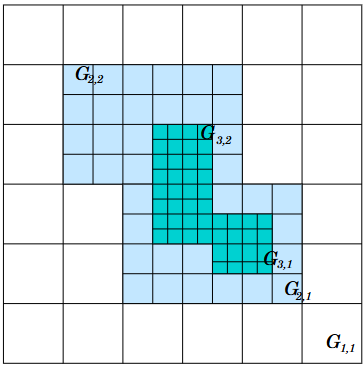
\includegraphics[width=\textwidth]{./imagens/Hierarquia_ilustrada.png}
    \caption{Ilustração da hierarquia de níveis utilizada no \textit{AMR}. Fonte; \cite{Villar2007}}
    \label{fig:ilustração_AMR}
\end{figure}

Nesse método, cada patch de malha é tratado como um elemento computacional separado, sendo que, em algumas implementações, cada nível de malha possui sua própria equação de discretização e seu próprio passo de tempo. Tais características fazem com que este seja um método otimizado do ponto de vista computacional, solucionando o problema de refinamento adaptativo com um custo computacional aceitável \citep{Ceniceros}.

O acoplamento entre os níveis pode ser feito de diversas formas e depende principalmente da estratégia de avanço temporal utilizado. Considerando que os níveis mais refinados, $l>l_1$, podem possuir faces que não tocam o domínio computacional, esses necessitam de condições de contorno adicionais que são fornecidas tanto pelos patches irmãos, que pertencem ao mesmo nível de refinamento, ou pelos níveis grosseiros, sendo que neste último caso o método varia por esquema utilizado. Os trabalhos originais de \citet{Berger1984} e \citet{Berger1989} focam em esquemas de discretização temporal explícitos para as equações de balanço de equações hiperbólicas, \citet{berger1989} utiliza interpolações bilineares dos níveis mais grosseiros para os mais finos e patches de malhas alinhadas aos eixos principais do domínio computacional. \citet{berger1991} melhora a eficiência dos patches e a forma com que eles são divididos, evitando redundâncias.

\citet{Roma1997} trabalhou juntamente com Berger e Peskin para utilizar a teoria de malha adaptativa para refinar a região próxima à superfície do método de immersed boundary, possibilitando a representação de geometrias elásticas e móveis em malha estruturada e adaptativa. Neste trabalho Roma utilizou polinômios interpoladores que utilizam informações tanto do nível que recebem as informações quanto do que fornece as mesmas, com um sistema de avança de forma semi-implícita no tempo. O método proposto por Roma utiliza o mesmo passo de tempo para todos os níveis, extendendo o passo de tempo do nível mais fino para todo o domínio. \citet{Vilar2007} aplicou a metodologia para escoamento bifásicos com a presença de dois fluidos, utilizando \textit{VOF} para representar os domínios, utilizando em seu trabalho passo de tempo fixo e os mesmos polinômios de Roma. \cite{Ceniceros} estendeu o trabalho para um domínio tridimensional totalmente adaptativo, utilizando o método phase-field para representar escoamentos bifásicos. 

Para este trabalho a adaptatividade do algoritmo descrito não foi utilizada, aproveitando-se a hierarquia de malhas aninhadas e a divisão do bloco de malhas em níveis. Como o código utilizado é herdado do trabalho de \citet{Villar2007} e originalmente o passo de tempo é fixo para todos os níveis. Como é mostrado em Seção (verificar a seção) os domínios simulados utilizam passo de tempos diferentes, sendo este um detalhe da implementação e não característica herdada. 

